\documentclass[a4paper]{article}

\usepackage[a4paper, lmargin=0.1666\paperwidth, rmargin=0.1666\paperwidth, tmargin=0.1111\paperheight, bmargin=0.1111\paperheight]{geometry} 

\usepackage{amsmath}
\usepackage{graphicx}
\usepackage{float}

\usepackage{tikz}
\usepackage{pgfplots}

\usetikzlibrary{shapes,arrows,positioning,calc}

\pgfplotsset{compat=newest}

\tikzset{
block/.style = {draw, fill=white, rectangle, minimum height=3em, minimum width=3em},
tmp/.style  = {coordinate}, 
sum/.style= {draw, fill=white, circle, node distance=1cm},
input/.style = {coordinate},
output/.style= {coordinate},
pinstyle/.style = {pin edge={to-,thin,black}}
}

\setlength\parindent{0pt}

\begin{document}

\begin{titlepage}

	\begin{center}
	
		\hrule \vspace{0.3cm} \huge{\textbf{Self-Balancing Bicycle}} \vspace{0.2cm} \\ \Large{Final Project} \vspace{0.2cm} \hrule 
						
		\vspace{3cm}
		
		\large{\textbf{Philip Salmony \\ Wolfson College \\ pms67@cam.ac.uk}}
		
		\vspace{2cm}
		
		\large{\textbf{Supervisor: Dr. Fulvio Forni}}		
		
		\vspace{2cm}		
		
		
\includegraphics[scale=0.15]{unilogo}
		
		\vspace{3cm}
		
		\large{4 September 2018}

	\end{center}

\vfill

\section*{Summary}
Modelling, analysis, simulation, and implementation of an autonomous, self-balancing bicycle.

\end{titlepage}

\newpage

\setcounter{page}{2}
\tableofcontents

\newpage

\section{Introduction and Objectives}

\begin{enumerate}
\item Autonomous self-balancing at close-to-zero forward velocity and above.
\item Robustness to modelling inaccuracies as well as to mass and geometry changes.
\item Trajectory tracking.
\end{enumerate}

\section{Notation}

Coordinate systems, notation(e.g. $m_{rf}$, $I_{xx}$, etc..)

\section{Bicycle Modelling}

\begin{figure}[H]
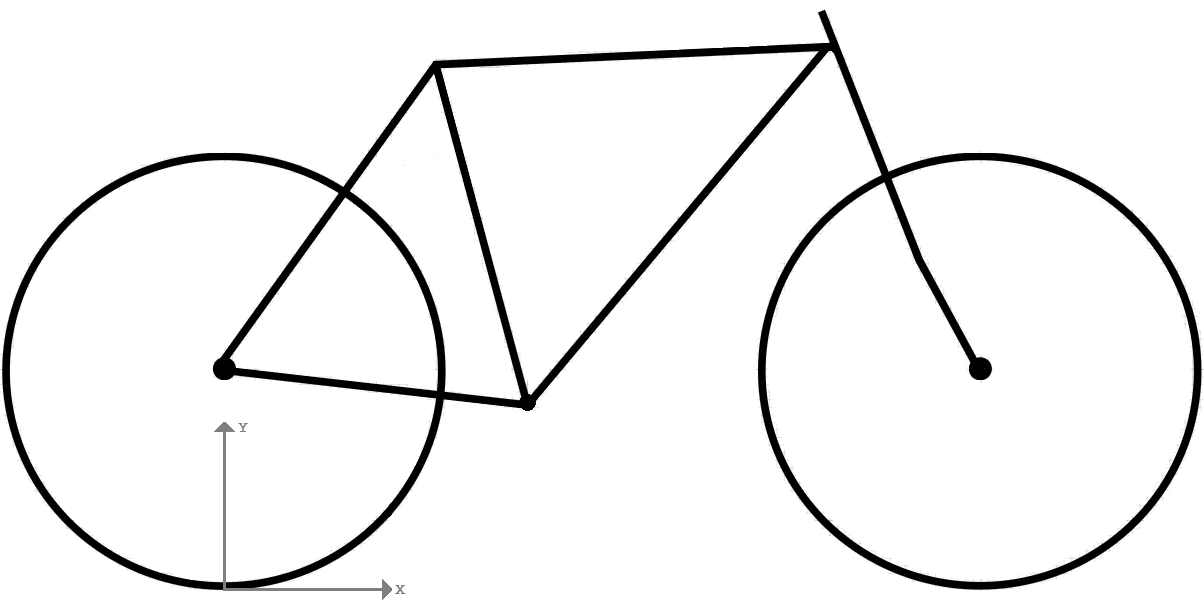
\includegraphics[scale=0.2]{BikeAxes}
\centering
\caption{Simplified Bike Model and Coordinate System}
\end{figure}

\subsection{Mass and Center of Mass}
The purchased bike was disassembled and the masses of both wheels and the remaining frame measured using a luggage scale. To estimate the masses of the rear and front frames, the dimensions of each connecting tube of the frames was measured to approximate their respective volumes. As mass is proportional to volume, this enabled an estimate of the individual masses of the tubes. Summing the tubes belonging to the appropriate frame gave an approximation of the mass of that frame. The results are as follows:

\begin{itemize}
\item $m_{rf} = 7.8 kg$
\item $m_{ff} = 2.1 kg$
\item $m_{rw} = 3.1 kg$
\item $m_{fw} = 2.5 kg$
\end{itemize}

\noindent \textbf{Rear Frame} \\
$(x, y, z)_{rf} = [0.507, 0.000, -0.534]$ \\

\noindent \textbf{Front Frame} \\
$(x, y, z)_{ff} = [0.960, 0.000, -0.597]$ \\

\noindent \textbf{Rear Wheel} \\
$(x, y, z)_{rw} = [0.000, 0.000, -0.320]$ \\

\noindent \textbf{Front Wheel} \\
$(x, y, z)_{ff} = [1.080, 0.000, -0.320]$

\subsection{Inertia Tensor}
The moment of inertia tensor describes the resistance to rotational motion of a three-dimensional object around certain axes about its center of mass. It is defined as follows,

\begin{equation*}
\mathbf{I} = 
\begin{pmatrix}
Ixx & Ixy & Ixz \\
Iyx & Iyy & Iyz \\
Izx & Izy & Izz
\end{pmatrix}.
\end{equation*}

\noindent We make the simplifying assumption that the terms $I_{xz}$, $I_{zx}$, $I_{yz}$, $I_{zy}$ are zero. The definitions for the remaining terms are,

\begin{align*}
I_{xx} &= \int (y^2 + z^2) dm \\
I_{yy} &= \int (x^2 + z^2) dm \\
I_{zz} &= I_{xx} + I_{yy} \\
I_{xy} &= I_{yx} = - \int (x \cdot y )dm
\end{align*}

\noindent \textbf{Rear Frame} \\
\begin{equation*}
\mathbf{I_{rf}} = \begin{pmatrix}
0.206 & 0 & 0.164 \\
0 & 0.643 & 0 \\
0.164 & 0 & 0.444
\end{pmatrix}
\end{equation*}

\noindent \textbf{Front Frame} \\
\begin{equation*}
\mathbf{I_{ff}} = \begin{pmatrix}
0.061 & 0 & -0.017 \\
0 & 0.059 & 0 \\
-0.017 & 0 & 0.013
\end{pmatrix}
\end{equation*}

\noindent \textbf{Rear Wheel} \\
\begin{equation*}
\mathbf{I_{rw}} = \begin{pmatrix}
0.159 & 0 & 0 \\
0 & 0.317 & 0 \\
0 & 0 & 0.159
\end{pmatrix}
\end{equation*}

\noindent \textbf{Front Wheel} \\
\begin{equation*}
\mathbf{I_{fw}} = \begin{pmatrix}
0.128 & 0 & 0 \\
0 & 0.256 & 0 \\
0 & 0 & 0.128
\end{pmatrix}
\end{equation*}

\subsection{Overall Description}

\textbf{Total System} \\

\noindent \textit{Mass and Center of Mass}
\begin{align}
m_t &= m_{rw} + m_{rf} + m_{ff} + m_{fw} = 15.5 \\
x_t &= \frac{1}{m_t} (x_{rf} m_{rf} + x_{ff} m_{ff} + w m_{fw}) = 0.559 \\
z_t &= \frac{1}{m_t} (-R_{rw} m_{rw} + z_{rf} m_{rf} + z_{ff} m_{ff} - R_{fw} m_{fw}) = -0.465
\end{align}

\noindent \textit{Moments and Products of Inertia}
\begin{align}
T_{xx} &= A_{xx} + B_{xx} + C_{xx} + D_{xx} + m_{rw} R^2_{rw} + m_{rf} z^2_{rf} + m_{ff} z^2_{ff} + m_{fw} R^2_{fw} = 4.10 \\
T_{xz} &= B_{xz} + C_{xz} - m_{rf} x_{rf} z_{rf} - m_{ff} x_{ff} z_{ff} + m_{fw} w R_{fw} = 4.33 \\
T_{zz} &= A_{zz} + B_{zz} + C_{zz} + D_{zz} + m_{rf} x^2_{rf} + m_{ff} x^2_{ff} + m_{fw} w^2 = 7.60
\end{align}

\noindent \textbf{Front Frame} \\

\noindent \textit{Mass and Center of Mass}
\begin{align}
m_f &= m_{ff} + m_{fw} = 4.6 \\
x_f &= \frac{1}{m_f} (x_{ff} m_{ff} + w m_{fw}) = 1.025 \\
z_f &= \frac{1}{m_f} (z_{ff} m_{ff} - R_{fw} m_{fw}) = -0.446
\end{align}

\noindent \textit{Moments and Products of Inertia}
\begin{align}
F_{xx} &= C_{xx} + D_{xx} + m_{ff} (z_{ff} - z_f)^2 + m_{fw} (R_{fw} + z_f)^2 = 0.277 \\
F_{xz} &= C_{xz} - m_{ff} (x_{ff} - x_f) (z_{ff} - z_f) + m_{fw} (w - x_f) (R_{fw} + z_f) = -0.0549 \\
F_{zz} &= C_{zz} + D_{zz} + m_{ff} (x_{ff} - x_f)^2 + m_{fw} (w - x_f)^2 = 0.157
\end{align}

\noindent \textbf{Miscellaneous} \\
\begin{align}
\lambda &= \frac{\pi}{2} - \alpha = \frac{\pi}{9}\\
u &= (x_f - w - t) \cdot cos(\lambda) - z_f \cdot sin(\lambda) = 0.021 \\
S_r &= \frac{A_{yy}}{R_{rw}} = 0.991, S_f = \frac{D_{yy}}{R_{fw}} = 0.800, S_t = S_r + S_f = 1.79
\end{align}

\section{Equations of Motion}

\subsection{Second Order Model}

\subsubsection{Excluding Fork Dynamics}

Simplified tilt equation:

\begin{equation}
\ddot{\theta} = \frac{Mgl}{J} sin(\theta) + \frac{Ml}{J} \Big( \frac{v^2_r}{b} tan(\phi) + \frac{a}{b} \frac{d(v tan(\phi))}{dt} \Big) cos(\theta)
\end{equation}

\noindent For near-upright motion with constant velocity $v$: $\dot{v} = 0$, $sin(\theta) \approx \theta$, $tan(\phi) \approx \phi$, and $cos(\theta) \approx 1$. We can therefore linearise the equation as follows:

\begin{equation}
\ddot{\theta} = \frac{Mgl}{J} \theta + \frac{Ml}{J} \Big( \frac{v^2}{b} \phi + \frac{a}{b} v \dot{\phi} \Big)
\end{equation}

\noindent Defining $\gamma = \frac{Ml}{Jb}$:

\begin{equation*}
\ddot{\theta} = b g \gamma \theta + \gamma (v^2_r \phi + a v \dot{\phi})
\end{equation*}

\noindent Taking Laplace transforms:

\begin{equation*}
s^2 \bar{\theta} = b g \gamma \bar{\theta} + \gamma (v^2_r \bar{\phi} + s a v \bar{\phi}) \\
\end{equation*}

\begin{equation*}
\bar{\theta} (s^2 - b g \gamma) = \bar{\phi} \gamma v (s a + v) 
\end{equation*}

\noindent Which results in the transfer function $G(s)$ from steer angle $\phi$ to lean angle $\theta$:

\begin{equation}
G(s) = \gamma v a \frac{(s + \frac{v}{a})}{(s^2 - b g \gamma)}
\end{equation}

\noindent We can extract three bits of information:

\begin{enumerate}
\item Gain: $k = \frac{M l v a}{J b}$
\item Zero: $z = -\frac{v}{a}$
\item Poles: $p_{1,2} = \pm \sqrt{\frac{M l g}{J}}$
\end{enumerate}

\noindent The gain tells us that as our forward velocity $v$ goes to zero, turning the forks will not influence the tilt angle. \\
The zero tells us that this is a minimum phase system. \\
The poles tell us that this system is unstable and non-oscillatory. \\

For the prototype bicycle the transfer function becomes,

\begin{equation}
G(s) = 0.491 \cdot v \cdot \frac{(s + \frac{v}{0.559})}{(s^2-9.30)}.
\end{equation}

\subsubsection{Including Fork Dynamics}

Shows stability for large enough forward speed...

\subsection{Fourth Order Model}

A model found in many research papers, is the fourth order linearised model consisting of two coupled second order differential equations. This model can be written in the following matrix form:

\begin{equation}
\mathbf{M} \cdot \underline{\ddot{q}} + [\mathbf{C_1} \cdot v] \cdot \underline{\dot{q}} + [\mathbf{K_0} + \mathbf{K_2} \cdot v^2] \cdot \underline{q} = \underline{f}
\end{equation}

Where $q = [\phi,  \delta]^T$ is a vector containing the lean angle ($\phi$) and the steer angle ($\delta$), $f = [T_{\phi}, T_{\delta}]^T$ is a vector consisting of a roll torque disturbance and handlebar torque, and finally the system matrices, which are derived from the bicycle geometry:

\begin{enumerate}
\item $\mathbf{M}$ - Mass matrix
\item $\mathbf{C_1}$ - Damping matrix, varying \textit{linearly} with velocity
\item $\mathbf{K_0}$ and $\mathbf{K_2}$ - Stiffness matrices, varying \textit{quadratically} with velocity
\end{enumerate}

The elements of each matrix are as follows:

\begin{equation}
\mathbf{M} = \begin{bmatrix}
T_{xx} & F_{\lambda x} + f T_{xz} \\
F_{\lambda x} + f T_{xz} & F_{\lambda \lambda} + 2 f F_{\lambda z} + f^2 T_{zz}
\end{bmatrix}
\end{equation}

\begin{equation}
\mathbf{C_1} = \begin{bmatrix}
0 & f S_t + S_f cos(\lambda) + T_{xz} \frac{cos(\lambda)}{w} - f m_t z_t \\
-(f S_t + S_f cos(\lambda)) & F_{\lambda z} \frac{\lambda}{w} + f (S_u + T_{zz} \frac{cos(\lambda)}{w}
\end{bmatrix}
\end{equation}

\begin{equation}
\mathbf{K_0} = \begin{bmatrix}
g m_t z_t & -g S_u \\
-g S_u & -g S_u sin(\lambda)
\end{bmatrix}
\end{equation}

\begin{equation}
\mathbf{K_2} = \begin{bmatrix}
0 & (S_t - m_t z_t) \frac{cos(\lambda)}{w} \\
0 & (S_u + S_f sin(\lambda)) \frac{cos(\lambda)}{w}
\end{bmatrix}
\end{equation}

\subsubsection{Decoupling and Transfer Functions}

Taking Laplace Transforms, assuming zero initial conditions:

\begin{equation*}
s^2 \cdot \mathbf{M} \cdot \underline{\bar{q}} + s \cdot [\mathbf{C_1} \cdot v] \cdot \underline{\bar{q}} + [\mathbf{K_0} + \mathbf{K_2} \cdot v^2] \cdot \underline{\bar{q}} = \underline{\bar{f}} 
\end{equation*}

\noindent Rearranging into transfer function form yields:

\begin{equation}
\mathbf{G}(s) = \Big(s^2 \cdot \mathbf{M} + s \cdot \mathbf{C_1} \cdot v + (\mathbf{K_0} + \mathbf{K_2} \cdot v^2) \Big)^{-1}
\end{equation}

\noindent Since $K_{2_{11}}=K_{2_{21}}=C_{1_{11}}=0$, the determinant of $\mathbf{G}(s)$ is

\begin{align*}
det(\mathbf{G}(s)) = P(s) &= s^4 \cdot (M_{11} M_{22} - M_{12} M_{21}) \\
&+ s^3 \cdot v \cdot (M_{11} C_{1_{22}} - (M_{12} C_{1_{21}} + M_{21} C_{1_{12}}) \\
&+ s^2 \cdot (M_{11} K_{0_{22}} + M_{22} K_{0_{11}} - M_{21} K_{0_{12}} - M_{12} K_{0_{21}}) + v^2 \cdot (M_{11} K_{2_{22}} - M_{21} K_{2_{12}} - C_{1_{12}} C_{1_{21}})) \\
&+ s \cdot v \cdot (K_{0_{11}} C_{1_{22}} - K_{0_{21}} C_{1_{12}} - K_{0_{12}} C_{1_{21}} - v^2 \cdot K_{2_{12}} C_{1_{21}}) \\
&+ (K_{0_{11}} K_{0_{22}} - K_{0_{21}} K_{0_{12}}) + v^2 \cdot (K_{0_{11}} K_{2_{22}} - K_{0_{21}} K_{2_{12}}).
\end{align*}

\noindent Where the roots of $P(s)$ are equal to the poles of the system. \\

\noindent As can be seen from the long expression above, it is hard to directly see what parameters in the bicycle's geometry - or the forward speed - influence the stability. This is especially true, since this is a linearised model of a much more complex system! \\

\noindent Continuing with the evaluation of the matrix inverse, we get a set of four decoupled transfer functions relating the roll and steer torque inputs to the roll and steer angular outputs: \\

\noindent \textit{(i) Roll Torque Disturbance to Lean Angle}
\begin{equation*}
G_{11}(s) = \frac{m_{22} \cdot s^2 + v \cdot C_{1_{22}} \cdot s + (K_{0_{22}} + K_{2_{22}} \cdot v^2)}{P(s)}
\end{equation*}

\noindent \textit{(ii) Roll Torque Disturbance to Steer Angle}
\begin{equation*}
G_{12}(s) = - \frac{m_{12} \cdot s^2 + v \cdot C_{1_{12}} \cdot s + (K_{0_{12}} + K_{2_{12}} \cdot v^2)}{P(s)}
\end{equation*}

\noindent \textit{(iii) Handlebar Torque to Lean Angle}
\begin{equation*}
G_{21}(s) = - \frac{m_{21} \cdot s^2 + v \cdot C_{1_{21}} \cdot s + K_{0_{21}}}{P(s)}
\end{equation*}

\noindent \textit{(iv) Handlebar Torque to Steer Angle}
\begin{equation*}
G_{22}(s) = \frac{m_{11} \cdot s^2 + K_{0_{11}}}{P(s)}
\end{equation*}

\noindent Again, it is hard to see how the bicycle parameters influence the positions of the systems zeros. \\

\noindent For the prototype bicycle the poles $P(s)$ are then given by,

\begin{equation}
P(s) = 0.711 s^4 + 1.30 v s^3 + s^2 (-22.3 + 5.01 v^2) + s v(-21.4 + 6.93 v^2) + (123 - 5.54 v^2)
\end{equation}

\noindent Which leads to following the set of transfer functions:

\noindent \textit{(i) Roll Torque Disturbance to Lean Angle}
\begin{equation}
G_{11}(s) = \frac{0.214 \cdot s^2 + v \cdot 0.744 \cdot s + (-2.48 + 0.881 \cdot v^2)}{P(s)}
\end{equation}

\noindent \textit{(ii) Roll Torque Disturbance to Steer Angle}
\begin{equation}
G_{12}(s) = - \frac{0.407 \cdot s^2 + v \cdot 5.18 \cdot s + (-7.25 + 7.83 \cdot v^2)}{P(s)}
\end{equation}

\noindent \textit{(iii) Handlebar Torque to Lean Angle}
\begin{equation}
G_{21}(s) = - \frac{0.407 \cdot s^2 - 0.884 \cdot v \cdot s - 7.25}{P(s)}
\end{equation}

\noindent \textit{(iv) Handlebar Torque to Steer Angle}
\begin{equation}
G_{22}(s) = \frac{4.10 \cdot s^2 - 70.7}{P(s)}
\end{equation}

\subsection{State Space Form}

Choosing states as $\underline{x} = \begin{bmatrix}
\phi & \delta & \dot{\phi} & \dot{\delta}
\end{bmatrix}^T$ and inputs as $\underline{u} = \begin{bmatrix}
T_{\phi} & T_{\delta}
\end{bmatrix}^T$ , we arrive at the following state space model for our prototype bicycyle (assuming all our states are measurable):

\begin{equation*}
\begin{gathered}
\underline{\dot{x}} = \mathbf{A} \underline{x} + \mathbf{B} \underline{u} \\
\underline{y} = \mathbf{C} \underline{x}
\end{gathered}
\end{equation*}

\noindent With the system matrices being,

\begin{equation}
\begin{gathered}
\mathbf{A} = \begin{bmatrix}
0 & 0 & 1 & 0 \\
0 & 0 & 0 & 1 \\
17.1 & 0.761 - 1.85 v^2 & -0.506 v & -1.13 v \\
1.36 & 10.2 - 0.602 v^2 & 5.10 v & -1.32 v
\end{bmatrix} \\
\mathbf{B} = \begin{bmatrix}
0 & 0 \\
0 & 0 \\
0.300 & -0.572 \\
-0.572 & 5.77
\end{bmatrix} \\
\mathbf{C} = \begin{bmatrix}
1 & 0 & 0 & 0 \\
0 & 1 & 0 & 0 \\
0 & 0 & 1 & 0 \\
0 & 0 & 0 & 1
\end{bmatrix}
\end{gathered}
\end{equation}

\section{Controller Design}

What can we actuate? What sensor do we have? Controllability/Observability

\subsection{Stability Analysis}

\subsubsection{Dependence on Forward Speed}

Three controller regimes.

\begin{figure}[H]
	\begin{tikzpicture}
		\begin{axis}
			[xlabel=Forward Speed $v$,
			 ylabel=Real Part of Eigenvalue $\lambda$,
			 xmin=0,xmax=6,
			 ymin=-10,ymax=5]
			\addplot[mark=none] table[x=v,y=a, col sep=comma] {StabilityVsForwardSpeed.csv};
			\addplot[mark=none] table[x=v,y=b, col sep=comma] {StabilityVsForwardSpeed.csv};
			\addplot[mark=none] table[x=v,y=c, col sep=comma] {StabilityVsForwardSpeed.csv};
			\addplot[mark=none] table[x=v,y=d, col sep=comma] {StabilityVsForwardSpeed.csv};
			
			\draw [dashed, thin] (0,0) -- (6,0);
			\draw [dotted, thin] (3,-10) -- (3,5);
			\draw [dotted, thin] (4.8,-10) -- (4.8,5);
		\end{axis}
	\end{tikzpicture}
	\centering
	\caption{Pole Locations vs Forward Speed}
\end{figure}

\subsection{Single Input Single Output (SISO)}

\textbf{CURRENTLY EXCLUDING FORK DYNAMICS - WILL CHANGE}

Which transfer function model do we use? Second order, fourth order, or both? BOTH

\subsubsection{Proportional Controller}

\begin{figure}[H]

	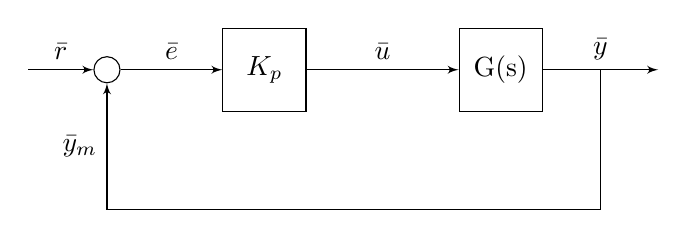
\begin{tikzpicture}[auto, node distance=2cm,>=latex']
		\node [input, name=input] {};
		\node [sum, right of=input] (sum) {};
		\node [block, right of=sum] (pcontr) {$K_p$};
		\node [block, right of=pcontr, node distance=3cm] (system) {G(s)};

		\draw [->] (pcontr) -- node[name=u] {$\bar{u}$} (system);
		\node [output, right of=system] (output) {};

		\coordinate [below of=u] (measurements) {};

		\draw [draw,->] (input) -- node {$\bar{r}$} (sum);
		\draw [->] (sum) -- node {$\bar{e}$} (pcontr);
		\draw [->] (system) -- node [name=y] {$\bar{y}$}(output);

		\draw [-] (y) |- (measurements);
		\draw [->] (measurements) -| node [near end] {$\bar{y}_m$} (sum);
    \end{tikzpicture}    
	\centering
	\caption{P Controller Structure}
\end{figure}

\textbf{Transfer Function} \\
Plotting the root locus diagram for the tilt transfer function, we can see that a simple proportional controller ($K(s) = K_p$) in a standard negative feedback configuration can stabilise this plant. The closed-loop transfer function $P(s)$ is of the following form:

\begin{equation}
P(s) = K_p \cdot (\gamma v a) \cdot \frac{(s + \frac{v}{a})}{s^2+ (\gamma v a) K_p s + \gamma (v^2_r K_p - b g)}
\end{equation}

\noindent Using the following root locus relationship to find the required proportional gain:

\begin{equation}
K_p = \frac{1}{\lvert G(s) \rvert}
\end{equation}

\noindent We are concerned with finding the minimum proportional gain that will guarantee closed-loop stability, therefore we wish to find a gain that will give us $s < 0$. Therefore, at $s = 0$, $Kp = \frac{b g}{v^2_r}$, which is the proportional gain needed for marginal stability. We require a gain larger than this to ensure asymptotic stability. \\

\noindent The furthest left we can go in the s-plane by increasing $K_p$ is when our closed-loop pole meets the open-loop zero at $\frac{v}{a}$, which gives an exponential decay time constant of $\frac{a}{v}$.

\textbf{Prototype Bicycle} \\
For the prototype bicycle, the closed-loop transfer function with a proportional controller becomes,

\begin{equation}
P(s) = 0.491 \cdot K_p \cdot v \cdot \frac{(s + \frac{v}{0.559})}{s^2 + 0.491 \cdot K_p \cdot v \cdot s + 0.878 \cdot (v^2 K_p - 10.6)}.
\end{equation}

From above, we require a minimum proportional gain of $K_p = \frac{bg}{v^2} = \frac{10.6}{v^2}$ for stability.

\subsubsection{P-D Controller}

\begin{figure}[H]

	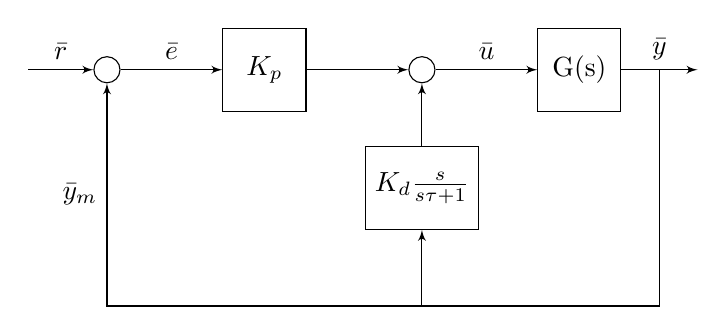
\begin{tikzpicture}[auto, node distance=1.5cm,>=latex']
		\node [input, name=input] {};
		\node [sum, right of=input] (sum1) {};
		\node [block, right of=sum1, node distance=2cm] (pcontr) {$K_p$};
		\node [sum, right of=pcontr, node distance=2cm] (sum2) {};
		\node [block, right of=sum2, node distance=2cm] (system) {G(s)};
	
		\node [block, below of=sum2, node distance=1.5cm] (dcontr) {$K_d \frac{s}{s \tau + 1}$};	
	
		\draw [->] (pcontr) -- (sum2);
		\draw [->] (sum2) -- node[name=u] {$\bar{u}$} (system);
		\node [output, right of=system] (output) {};

		\coordinate [below of=dcontr] (measurements) {};
		\draw [->] (dcontr) -- (sum2);
		\draw [->] (measurements) -- (dcontr);

		\draw [draw,->] (input) -- node {$\bar{r}$} (sum1);
		\draw [->] (sum1) -- node {$\bar{e}$} (pcontr);
		\draw [->] (system) -- node [name=y] {$\bar{y}$}(output);

		\draw [-] (y) |- (measurements);
		\draw [->] (measurements) -| node [near end] {$\bar{y}_m$} (sum1);
    \end{tikzpicture}    
	\centering
	\caption{P-D Controller Structure}
\end{figure}

Derivative on measurement to avoid \textit{derivative kick} when setpoint changes. \\

\textbf{Derivative on Measurement} \\
e = r - y \\
u = $K_p$ * e - Kd * s / (sT + 1) * y \\
y = G * u \\

\textbf{Band-Limited Differentiator} \\
Since a pure differentiator acts as an amplifier for high frequencies, it will also amplify any high-frequency noise present in the measured plant output. Additionally, for a low sample time, this amplification increases by $\frac{1}{T}$. This will result in extreme \textit{jittering} of the actuator, drastically reducing its lifespan and the overall control performance. Furthermore, we cannot calculate the exact derivative at time $t$. We need to approximate it numerically, for example, using Euler's backward difference method. \\
To address these problems, instead of implementing a pure derivative controller with transfer function $s$, we utilize a band-limited differentiator. This is effectively a pure differentiator cascaded with a single-pole low-pass filter,

\begin{equation}
D(s) = K_d \frac{s}{s \tau + 1}, \qquad \tau > 0.
\end{equation}

Where $K_d$ is the associated derivative gain and $\tau$ is the filter time constant. The cut-off frequency (in $rads^{-1}$) of the low-pass filter is therefore $\frac{1}{\tau}$. The closer $\tau$ is to zero, the closer our approximation is to the actual derivative. However, we will also greatly increase our noise since this is inversely proportional to the cut-off frequency of the filter.

\begin{figure}[H]	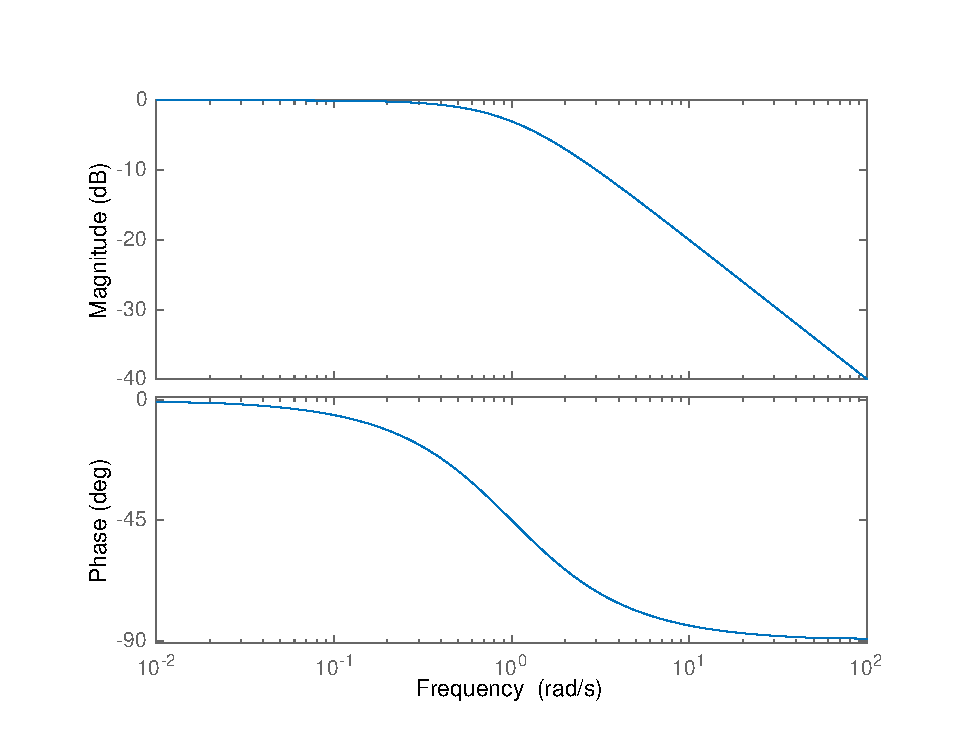
\includegraphics[scale=0.7]{BodeBandlimitedDiff}
\centering
\caption{Bode Diagram of Band-Limited Differentiator ($\tau = 1$)}
\end{figure}

% MATLAB: print -depsc -tiff -r300 -painters <filename>

\textbf{Transfer Function} \\
The closed-loop transfer function of the P-D controller in combination with a general plant $G(s)$ is thus,

\begin{equation*}
H(s) = \frac{K_p \cdot G(s)}{1 + G(s) \cdot (K_p + K_d \frac{s}{s \tau + 1})}.
\end{equation*}

Replacing $G(s)$ with the transfer function of the linearised second order bicycle model, we arrive at the following closed-loop transfer function:

\begin{equation}
H(s) = K_p \cdot \gamma v a \cdot \frac{(s + \frac{v}{a})}{s^2 - b g \gamma + \gamma v a \cdot (s + \frac{v}{a}) \cdot (K_p + K_d \frac{s}{s \tau + 1})}
\end{equation}

Where the transfer function can be further expanded by multiplying the numerator and denominator by $(s \tau + 1)$ to yield,

\begin{equation*}
H(s) = K_p \cdot \gamma v a \cdot \frac{(s+\frac{v}{a}) (s + \frac{1}{\tau})}{s^3 + s^2 \frac{1}{\tau} (1 + \gamma v a K_p \tau + K_d) + s \frac{\gamma}{\tau} (K_p v (a + v \tau) + K_d v^2 - b g \tau) + \frac{\gamma}{\tau} (v^2 K_p - b g)}.
\end{equation*}

For analysis and control design purposes, this equation is too complex. We therefore simplify the transfer function by assuming we filter the sensor measurements with the low-pass filter ($LP(s)=\frac{1}{s \tau + 1}$) before feeding them into the derivative-part of the controller. Therefore, we can assume a pure differentiator. This results in the simplified closed-loop, second order transfer function:

\begin{align*}
H^*(s) &= K_p \cdot \gamma v a \cdot \frac{(s + \frac{v}{a})}{s^2 (1 + K_d \gamma v a) + s \gamma v (a K_p + v K_d) + \gamma (v^2 K_p - b g)} \\
&= \frac{K_p \gamma v a}{1 + K_d \gamma v a} \cdot \frac{(s + \frac{v}{a})}{s^2 + s \frac{\gamma v (a K_p + v K_d)}{1 + K_d \gamma v a} + \frac{\gamma (v^2 K_p - b g)}{1 + K_d \gamma v a}}
\end{align*}

\textbf{Pole Placement} \\
We need to place two poles for the closed-loop system ($p_1$ and $p_2$). The second-order characteristic equation is therefore,

\begin{equation*}
C(s) = (s - p_1) (s - p_2) = s^2 - (p_1 + p_2) s + p_1 p_2
\end{equation*}

To get the the controller gains $K_p$ and $K_d$ we equate the coefficients of the transform variable $s$ of the closed-loop transfer function's denominator with those of the characteristic equation:

\begin{align}
\frac{\gamma v (a K_p + v K_d)}{1 + K_d \gamma v a} &= -(p_1 + p_2) \\
\frac{\gamma (v^2 K_p - b g)}{1 + K_d \gamma v a} &= p_1 p_2
\end{align}

After rearranging, we arrive at the following matrix set of linear relationships for $K_p$ and $K_d$:

\begin{equation}
\begin{pmatrix}
\gamma v^2 & -\gamma v a p_1 p_2 \\
\gamma v a & \gamma v (v + (p_1 + p_2) a) 
\end{pmatrix}
\begin{pmatrix}
K_p \\ K_d
\end{pmatrix}
=
\begin{pmatrix}
p_1 p_2 + \gamma b g \\
-(p_1 + p_2)
\end{pmatrix}
\end{equation}

These can then be easily solved to give $K_p$ and $K_d$, so that:

\begin{equation*}
\begin{pmatrix}
K_p \\ K_d
\end{pmatrix}
=
\frac{1}{\gamma^2 v^2 (v(v + (p_1 + p_2) a) + a^2 p_1 p_2)}
\begin{pmatrix}
\gamma v (v + (p_1 + p_2) a) & \gamma v a p_1 p_2 \\
-\gamma v a & \gamma v^2
\end{pmatrix}
\begin{pmatrix}
p_1 p_2 + \gamma b g \\
-(p_1 + p_2)
\end{pmatrix}
\end{equation*}

\subsection{State Feedback}
Pole placement - do not want to drastically change system dynamics - essentially only want to provide stability (all real parts of eigenvalues must be negative). Can push poles further left in the s-plane to increase stability margins, especially since plant is modelled only approximately so will contain variations. Must watch that we do not hit the actuator limits by choosing poles magnitudes too large. \\
Gain-scheduled state feedback depending on forward velocity. Lookup tables, since computing poles is too resource intensive for microcontroller.

\subsection{Optimal Control}

\subsection{Zero-Speed Stabilisation}

\section{Trajectory Tracking}

\section{Simulation}

\subsection{MatLAB}

\subsection{Unity}

\section{Implementation}

Bike, Sensors, Actuators, System as a whole, Arduino, processing (LP Filter), complementary filter, kalman filter, IMU, post-processing (C\#/Python?), MatLAB, etc.

\section{Results and Discussion}

\section{Conclusions}



\section{References}

\section{Appendix}

\end{document}